\noindent\textbf{Concurrency in Device Drivers. }
%
Modern operating systems address the demand for responsiveness and performance in device drivers by providing multiple sources of concurrency~\cite{corbet2005linux}: the kernel can invoke an arbitrary number of entry points from the same driver concurrently; a running driver process can block and be replaced by another process in the same driver; and hardware interrupts can be handled concurrently.  These forms of concurrent execution are prone to \emph{data races}.

\begin{definition}
\label{definition:datarace}
A \emph{data race} occurs when two distinct threads access a shared memory location, at least one of the accesses modifies the location, at least one of the accesses is non-atomic, and there is no mechanism in place to prevent these accesses from being simultaneous.
\end{definition}

Figure~\ref{fig:data_race_example} shows a racy entry point, \texttt{nvram\_llseek}, in the generic\_nvram Linux driver. The driver can invoke the entry point concurrently from two threads $T_1$ and $T_2$, with the same \texttt{file} struct as a parameter. However, this can lead to multiple possible data races, because $T_1$ and $T_2$ can access the \texttt{f\_pos} field of \texttt{file} in arbitrary order. Our tool, \whoop (see \S\ref{whoop}), was able to find these races automatically (see \S\ref{evaluation}).

\begin{figure}[t]
\begin{lstlisting}
static loff_t nvram_llseek(struct file *file,
    loff_t offset, int origin) {
  switch (origin) {
    case 0: break;
    case 1: offset += file->f_pos; break; // racy
    case 2: offset += nvram_len; break;
    default: offset = -1;
  }
  if (offset < 0)
    return -EINVAL;
  file->f_pos = offset; // racy
  return file->f_pos; // racy
}
\end{lstlisting}
\vspace{-2mm}
\caption{Racy entry point in the generic\_nvram Linux driver}
\label{fig:data_race_example}
\end{figure}

The most common method for avoiding races is by protecting sets of program statements that access a shared resource using \emph{locks}, forming \emph{critical sections}.  Figure~\ref{fig:lock_example} shows how to use a lock to eliminate the races in Figure~\ref{fig:data_race_example}. Because the return statement can potentially race on the \texttt{f\_pos} field, we store the result in a temporary variable inside the critical section.
%
Careless use of locks has many well-known pitfalls~\cite{sutter2005software}: coarse-grained locking can hurt performance, as it limits the opportunity for concurrency; while fine-grained locking can easily lead to deadlocks. Although the Linux kernel provides sophisticated lock-free synchronization mechanisms~\cite{corbet2005linux}, such as atomic read-modify-write operations, in this work we focus on locks as they are widely used.\footnote{We treat lock-free operations soundly, by not regarding them as providing any protection between threads, but this can lead to false alarm race reports.}

\begin{figure}[t]
\begin{lstlisting}
static loff_t nvram_llseek(struct file *file,
    loff_t offset, int origin) {
  mutex_lock(&nvram_mutex); // lock
  switch (origin) {
    case 0: break;
    case 1: offset += file->f_pos; break;
    case 2: offset += nvram_len; break;
    default: offset = -1;
  }
  if (offset < 0)
    return -EINVAL;
  file->f_pos = offset;
  loff_t res = file->f_pos; // store result
  mutex_unlock(&nvram_mutex); // unlock
  return res;
}
\end{lstlisting}
\vspace{-2mm}
\caption{Using a lock to eliminate the data races in the previous example}
\label{fig:lock_example}
\end{figure}

\noindent\textbf{Lockset Analysis. }
%
Lockset analysis is a lightweight race detection method proposed in the context of Eraser~\cite{savage1997eraser}, a dynamic data race detector.  The idea is to track the set of locks that are \emph{consistently} used to protect a memory location during program execution. If that lockset ever becomes empty, the analysis reports a \emph{potential} race on that memory location. This is because an empty lockset suggests that a memory location \emph{may} be accessed simultaneously by two or more threads.  

Lockset analysis for a concurrent program starts by creating a \emph{current} lockset, $\mathit{CLS}_T$, for each thread $T$ of the program, and a lockset, $\mathit{LS}_s$, for each shared variable $s$ used in the program. Initially, $\mathit{CLS}_T$ is empty for every thread $T$, because the threads do not hold any locks on program start. The lockset $\mathit{LS}_s$ for each variable $s$ is initialized to the set of all locks manipulated by the program, because initially each access to $s$ has (vacuously) been protected by every lock. The program is executed as usual (with threads scheduled according to the OS scheduler), except that instrumentation is added to update locksets as follows.
%
After each \emph{lock} and \emph{unlock} operation by $T$, $\mathit{CLS}_T$ is updated to reflect the locks currently held by $T$.
%
When $T$ accesses shared variable $s$, any locks that are not common to $\mathit{LS}_s$ and $\mathit{CLS}_T$ are removed from $\mathit{LS}_s$.
If $\mathit{LS}_s$ becomes empty as a result, a warning is issued that the access to $s$ may be unprotected.

Figure~\ref{fig:locksets} shows an example of applying lockset analysis on a concurrent program consisting of two threads $T_1$ and $T_2$, both accessing a global variable $A$. Initially, $\mathit{LS}_A$, which is the lockset for A, contains all possible locks in the program: $M$ and $N$. During execution of $T_1$, the thread writes $A$ without holding $N$, and thus $N$ is removed from $\mathit{LS}_A$. Next, during execution of $T_2$, the thread writes $A$ without holding $M$, and thus $\mathit{LS}_A$ becomes empty. As a result, a warning is reported because the two threads do not consistently protect $A$.

In contrast to more sophisticated race analyses that encode a \emph{happens-before} relation between threads~\cite{lamport1978time} (e.g.\ using vector clocks), lockset analysis is easy to implement, lightweight, and thus has the potential to scale well.  The technique, though, suffers from imprecision (i.e.\ can report false bugs), because a violation of the locking discipline does not always correspond to a real data race~\cite{savage1997eraser, pozniansky2003efficient, o2003hybrid, elmas2007goldilocks, flanagan2009fasttrack}. Furthermore, the code coverage in dynamic lockset analyzers, such as Eraser, is limited by the execution paths that are explored under a given scheduler. This is because the tool runs the program in a truly concurrent environment, thus it only gets to see what the thread did on the particular schedule that was followed.

To counter the above limitations, techniques such as Locksmith~\cite{pratikakis2006locksmith} and RELAY~\cite{voung2007relay} have explored the idea of applying lockset analysis in a static context, using dataflow analysis. In this paper, we present a novel symbolic lockset analysis method that involves generating verification conditions, which are then discharged to a theorem prover.

\begin{figure}[t]
\centering
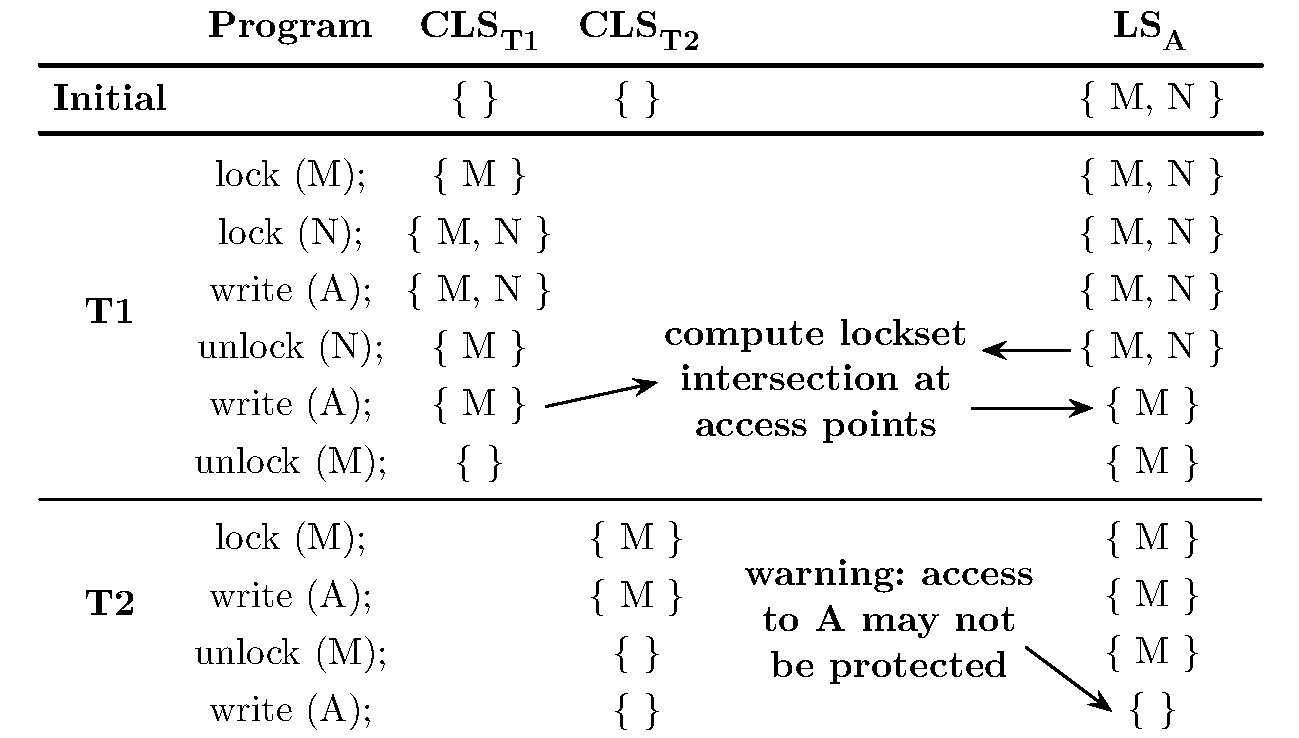
\includegraphics[width=1\linewidth]{img/lockset.pdf}
\caption{Applying lockset analysis on a concurrent program}
\label{fig:locksets}
\end{figure}
